% !TEX encoding = IsoLatin
\documentclass[12pt, a4paper]{article}
\usepackage[utf8]{inputenc}
\usepackage[T1]{fontenc}
%\usepackage[latin1]{inputenc}
\usepackage[hmargin = 25mm, vmargin = 25mm]{geometry}
%\geometry{letterpaper}                   % ... or a4paper or a5paper or ... 
%\geometry{landscape}                % Activate for for rotated page geometry
%\usepackage[parfill]{parskip}    % Activate to begin paragraphs with an empty line rather than an indent
\usepackage{graphicx}
\usepackage{amssymb, amsmath, amsthm}
\usepackage{epstopdf}
\usepackage{moreverb}
\usepackage{hyperref}
\usepackage{algorithm,algorithmic}
\usepackage[french]{babel}
\usepackage{hyperref}
\usepackage{fancyhdr} 
\usepackage{float}
\pagestyle{fancy}

\renewcommand{\headrulewidth}{0pt}
\fancyhead[C]{} 
\fancyhead[L]{}
\fancyhead[R]{}

\renewcommand{\footrulewidth}{0pt}
\fancyfoot[C]{\footnotesize{$13^{es}$ Journées de méthodologie statistique de l’Insee (JMS) / 12-14 juin 2018 / PARIS}}
\fancyfoot[R]{\thepage}

\begin{document}

\begin{center}

\includegraphics[width=15cm]{head_jms2018.png} 
\line(1,0){450}
\vspace{5mm}
\textbf{{\huge \'E}\Large LABORATION D'UNE MAILLE GEOGRAPHIQUE POUR L'HABITAT}
\end{center}

\begin{center}
\textit{Solène COLIN(*), Vivien ROUSSEZ(*)} \\
%- N. B. le premier nom doit être celui de l'auteur qui effectuera la présentation orale (sauf contributions associées)
\vspace{2mm}
\textit{(*) CGDD, Service de la Donnée et des \'Etudes Statistiques}\\ 

\vspace{2mm}
\url{solene-c.colin@developpement-durable.gouv.fr} \url{vivien.roussez@developpement-durable.gouv.fr} 
\end{center}
\vspace{5mm}
\small{{\bf Mots-cl\'es.} Analyse spatiale, graph mining, clustering, analyse multidimensionnelle, cartographie.}

\begin{center}
\line(1,0){450}
\end{center}


\section*{Résumé}

Le SDES a lancé en 2017 un projet visant à construire un maillage du territoire à même de rendre compte des disparités territoriales sur les enjeux propres au logement. En effet, ni les échelles administratives, ni les zonages d'études de l'Insee (zones d'emploi, bassins de vie) ne sont adaptées pour l'analyse localisée du logement, car ils mêlent dans les mêmes mailles des types d'habitat différents (urbain et périurbains notamment). Pour cela, neuf indicateurs représentatifs de l'équilibre des marchés du logement ont été sélectionné pour alimenter la méthode de \textbf{régionalisation}, qui regroupe les communes en bassins homogènes. La méthode retenue est l'algorithme \textbf{SKATER} (Spatial Klustering Analysis by Tree Edge Removal), qui s'appuie sur l'exploration de graphe et notamment la notion d'arbre portant minimal. \\

Différentes simulations ont été menées pour déterminer la taille de ces mailles, et les résultats ont fait l'objet de tests au niveau régional. Ces mailles mettent au premier plan les disparités propres au logement (pouvoir d'achat immobilier, taille des ménages), alors que la maille communale fait principalement ressortir les disparités liées au degré d'urbanité. Elle permet également de distinguer les villes-centre de leur périphérie, et donc d'isoler les enjeux propres à ces espaces très différents sur le plan du logement. \\

L'analyse de ces mailles permet de mettre en exergue six types de marchés locaux du logement, principalement distingués par le niveau des prix, la composition des ménages (leur taille) et du parc de logement. Au fil du temps, les spécificités de ces marchés se renforcent et ceux déjà en tension voient leurs déséquilibres se renforcer. A l'inverse, le ralentissement démographique et le vieillissement à l'\oe uvre dans les espaces faiblement peuplés contribuent à la faible dynamique des marchés où la demande est déjà modérée. Par ailleurs, ces marchés présentent un degré inégal d'homogénéité, et on trouve d'avantage de diversité entre les communes de marchés de l'Est de la France.

\section*{Abstract}

Partant du constat que les mailles géographiques usuelles ne permettent pas une analyse fine des marchés du logement, le SDES a élaboré une maille ad hoc. Pour cela, 9 indicateurs emblématiques de la demande et de l'offre des marchés locaux du logement ont été sélectionnés et ont alimenté une méthode de \textbf{régionalisation} utilisant la théorie des graphes et les arbres portants minimaux. Ce maillage permet une lecture facilitée des dynamiques territoriales sur les plans du logement et de la démographie.


\section*{Introduction}

Les mailles habitat constuites par le SDES ont pour objectif de constituer une échelle pertinente pour l'observation et l'analyse des enjeux territoriaux liés à l'habitat. Elle permet de répondre à trois objectifs :

\begin{itemize}
\item Lisser visuellement l'information pour donner des cartes lisibles
\item Conserver au maximum les disparités territoriales, tout en faisant ressortir les enjeux propres à l'habitat
\item Alimenter la connaissance et les diagnostics locaux
\end{itemize}


Pour cela, le SDES a construit des ensembles de communes qui \emph{se ressemblent} sur le domaine de l'habitat. Cette approche diffère de celle de l'Insee qui, pour ses zonages d'études, regroupe les communes qui sont fortement connectées les unes aux autres. Ce degré de connexion s'apprécie à l'aune du nombre de navettes domicile-travail entre les communes (pour les zones d'emploi) et les flux (théoriques) d'habitant se déplaçant de leur commune de résidence vers le pôle de services le plus proche (pour les bassins de vie). Pour plus d'information sur les maillages produits par l'Insee, consultez \href{https://www.insee.fr/fr/information/2114631}{cette page}.

\section{Sélectionner les indicateurs pertinents}

Choisis dans le cadre de deux comités regroupant des experts des territoires et du logement, les 9 indicateurs mobilisés sont représentatifs des marchés du logement, à la fois dans l'offre, la demande, et les équilibres de marché.

\subsection{Quels indicateurs}

Ces indicateurs sont calculés à partir de trois sources : recensements de la population, Filocom (Fichier des Logements localisés à la Commune), bases notariales (PERVAL et BIEN). Certaines communes ne présentant pas de donnée pour un ou plusieurs indicateurs, une \textbf{imputation} a été réalisée en prenant (de façon spatialement récursive) la moyenne de cet indicateur sur les communes voisines. Ces indicateurs sont présentés en détail dans le rapport méthodologique disponible sur le site internet du SDES.

\begin{enumerate}
\item L'indicateur de jeunesse du parc : part des logement récents (construits après 1975) rapportés à la part des logements anciens (construits avant 1949). 
\item Durée d'occupation médiane des logements
\item Taux de transactions dans le marché de l'ancien (nombre de transactions rapporté au nombre de logements)
\item Part de logements sociaux
\item Part de logements en situation de suroccupation
\item Prix au $m^2$ dans l'ancien rapportés au revenu médian communal, qui peut être analysé comme le nombre d'années de revenu nécessaires pour acheter 1 $m^2$
\item Nombre de personnes par ménage
\item Part des résidences secondaires
\item Part de logements vacants
\end{enumerate}


\begin{figure}[H]
\caption{ACP sur les indicateurs retenus}
\begin{center}
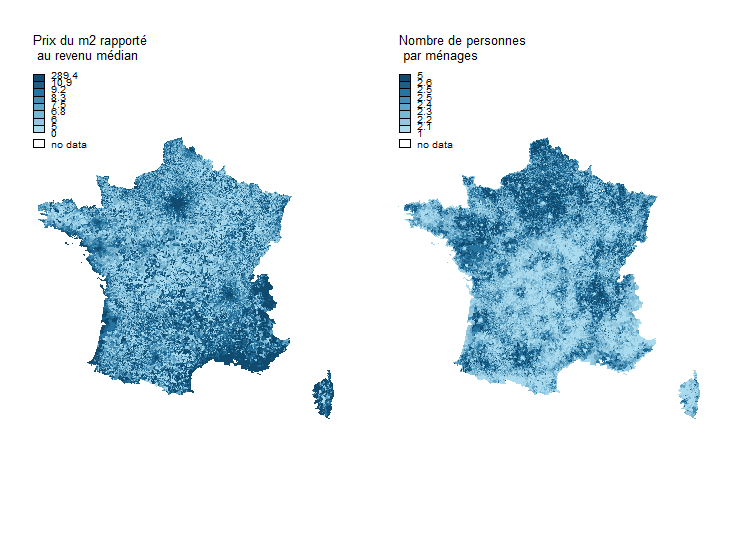
\includegraphics[scale=.8]{img/Indic_comm.png}
\end{center}
\end{figure}
\emph{Sources : calculs SDES d'après BIEN et PERVAL 2012, Filocom2013 et Insee, RP2014}
\subsection{Validation des indicateurs}

\subsubsection{Analyse en composantes principales}

Pour valider le choix des indicateurs sélectionnés (plusieurs itérations ont été nécessaires), une analyse en composantes principales (ACP) a été réalisée sur la base des indicateurs retenus. L'objectif consistait à retenir un minimum d'indicateurs pertinents et surtout \textbf{non redondants}, mais en conservant également quelques mesures "incontournables" de l'état du marché du logement (la part de logements sociaux, notamment).


\begin{figure}[H]
\caption{ACP sur les indicateurs retenus}
\begin{center}
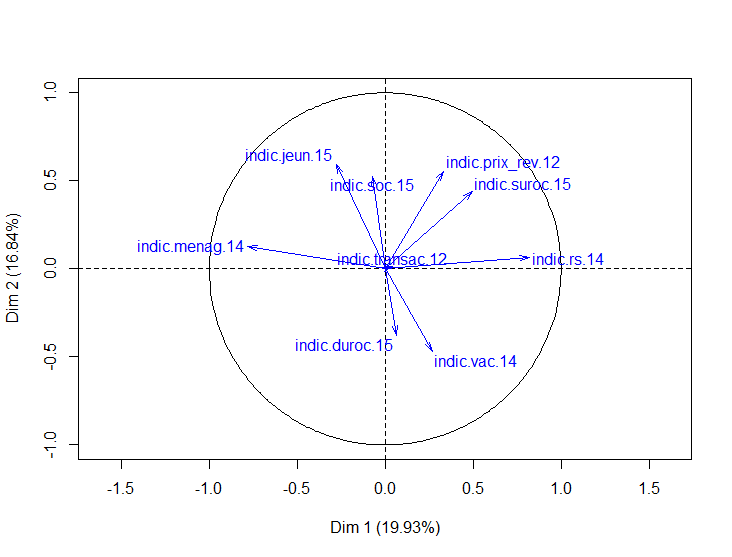
\includegraphics[scale=.7]{img/ACP.png}
\end{center}
\end{figure}
\emph{Source : calculs SDES}

Les résultats de l'ACP montrent que les indicateurs ne présentent pas de redondance d'information, ce qui aurait pu conduire à sur-pondérer une dimension (le clivage urbain / rural par exemple). Les 6 axes retenus permettent de mettre en lumière un certain nombre de caractéristiques territoriales, résumées dans le tableau suivant : \\

\begin{figure}[H]
\caption{Principaux axes factoriels}
\begin{tabular}{| l | l | c | l |}
\hline
Axe factoriel & Variables constitutives       & Signe &  Disparités territoriales révélées \\
\hline
Axe 1         &Jeunesse du parc               & +    & Gradient urbain \\
              &  Taille des ménages             & +  &    \\
\hline
Axe 2         &Prix                           & +    & Gradient de tension \\
       & Suroccupation                  & +    & \\ 
      &Taille des ménages             & -  &   \\
\hline
Axe 3         &Vacance                        & -    & Zones touristiques \\
        &Logements sociaux              & -    &  \\
        &Durée d'occupation             & +    & \\
\hline
Axe 4         &Taux de transactions           & +    & Coeurs des AU  \\
                                           &  & & Marchés dynamiques de l'Ouest et du Nord \\
\hline
Axe 5         &Durée d'occupation             & +    & Zones Nord-Est (propriétaires) \\
        &Social                         & +    & versus Sud et Sud-Est \\
\hline
Axe 6         & Suroccupation                  & +    & Couronnes périurbaines et \\
                 & &                &  zones touristiques du Sud-Est \\
\hline
\end{tabular}
\end{figure} 

\vspace{.2cm}


\subsubsection{Classification communale}


Par la suite, on effectue une classification des communes par centres mobiles, opérée sur les coordonnées factorielles des 6 premiers axes. Cette classification permet de mettre en exergues six groupes de communes qui permettent de rendre compte des principales disparités territoriales attendues. 
\begin{enumerate}
\item La classe 1 est la classe la plus proche de la moyenne sur l'ensemble des dimensions. Le parc y est toutefois légèrement plus récent que la moyenne, ainsi qu'une taille des ménages nettement supérieure à la moyenne. Elle correspond principalement aux communes des couronnes périurbaines de aires urbaines ;
\item La classe 2 présente le parc le plus ancien. Elle se démarque démarque également par une durée d'occupation plus importante. Elle est composée de communes distribuées le long de la diagonale nord-est/sud-est.
\item La classe 3 présente un taux de vacance relativement important, et des prix de l'immobilier les plus modérés. On y trouve les communes peu denses situées dans les espaces interstitiels du réseau urbain ;

\begin{figure}[H]
\caption{Classification des communes}
\begin{center}
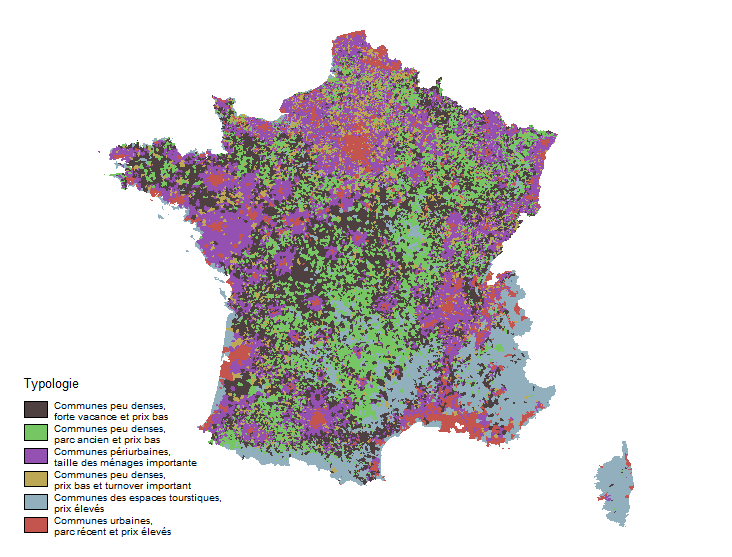
\includegraphics[scale=.7]{img/Typo_com.png}
\end{center}
\end{figure}
\emph{Source : calculs SDES}

\item La classe 4 correspond aux marchés les plus tendus : elle se détache sur le deuxième axe factoriel. Le parc de logement de cette classe est putôt récent et la proportion de logements sociaux y est élevée (ils sont d'ailleurs concentrés dans cette classe). La durée d'occupation y est également légèrement plus élevée que la moyenne. On y trouve principalement des espaces urbains avec les villes-centre des principales aires urbaines, ainsi que les espaces littoraux de la Méditerranée et de l'Atlantique.
\item La classe 5 présente des prix relativement élevés, mais un parc très différent, puisque plus ancien et comptant davantage de résidences secondaires. il s'agit de communes correspondant aux espaces touristiques, notamment des zones de montagne.
\item La classe 6 est principalement marquée par un taux de transaction relativement élevé, mais dans des marchés peu tendus, et dont le parc est relativement ancien. Il s'agit de communes de faible de densité démographique, essentiellement située dans le Nord du pays.
\end{enumerate}


Ces types sont cohérents avec d'autres études déjà réalisées, soit sur la dimension territoriale, soit sur  le logement. Ils confirment le choix des indicateurs qui a été fait. C'est donc sur cette base qu'est faite la régionalisation.


\section{La régionalisation}

La \textbf{régionalisation} désigne l'opération qui consiste à regrouper des unités géographiques élémentaires en un ensemble \textbf{contigu}, selon des critères statistiques. Il existe un grand nombre de méthodes de régionalisation, dont une partie est comparée dans \href{http://journals.sagepub.com/doi/pdf/10.1177/0160017607301605}{cet article}. Le SDES a retenu l'algorithme SKATER (Spatial Klustering Analysis by Tree Edge Removal), implémenté et mis à disposition dans le package \textsc{spdep} du logiciel statistique libre\textsc{R}.

\subsection{L'algorithme SKATER}

Cet algorithme fonctionne en 4 étapes :

\begin{enumerate}
\item Construction de la matrice de contiguïté $\rightarrow$ obtention d'un \emph{graphe} (un noeud = une commune et un lien = relation de contiguïté entre deux communes)
\item Pondération de ce graphe avec les dissimilarités calculées à partir des indicateurs (distance euclidienne)

\begin{figure}[H]
\caption{Illustration des étapes de SKATER sur les Hauts de Seine}
\begin{center}
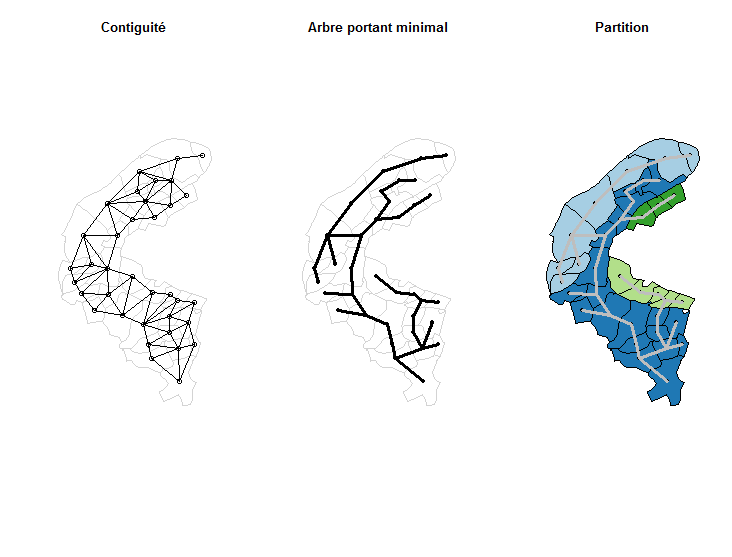
\includegraphics[scale=.7]{img/SKATER.png}
\end{center}
\end{figure}
\emph{Source : calculs SDES}

\item Construction de l'\textbf{arbre} portant minimal, en retenant le lien avec le voisin le plus ressemblant pour chaque n\oe ud du graphe
\item Suppression itérative des branches de l'arbre maximisant la variance inter-classes des sous-graphes obtenus après élagage.
\end{enumerate}

Il peut donc être vu comme une forme de classification descendante hiérarchique opérée sur les liens de l'arbre portant minimal. Le fait de travailler à partir de cet arbre portant minimal plutôt que sur les n\oe uds du graphe garantit la contiguïté des mailles finales.


\subsection{Découper le problème}

Cet algorithme est très couteux : sa complexité est en effet supérieure à $o(n^2)$, et il n'a pas été optimisé dans un langage plus efficace que R. En conséquence, il est impossible de traiter les près de 36000 communes françaises. En effet, le traitement de l'Île-de-France (moins de 1300 communes) prend environ 5 minutes, alors qu'il faut 3 heures pour le Grand-Est (environ 5000 communes). C'est pourquoi l'algorithme a été exécuté région par région. Toutefois, pour s'affranchir de ces limites administratives, on procède ensuite à un \emph{lissage} des frontières régionales. Pour cela, on identifie les mailles qui touchent une frontière régionale et on refait un zonage à partir de l'ensemble des communes qui appartiennent à ces espaces.\\
L'ordre de grandeur du nombre de communes qui se trouvent dans les zones concernées est de 16 000. La difficulté liée au temps de calcul apparaît donc de nouveau. Pour contourner ce problème, il faut découper cet ensemble en plusieurs sous-ensembles de taille plus petite. Pour réaliser ce découpage, on a repéré le barycentre du pays. La zone se trouvant sur ce barycentre, ainsi que les zones contiguës constituent une première \emph{macro-zone}.



\begin{figure}[H]
\caption{Répartition des mailles frontalières}
\begin{center}
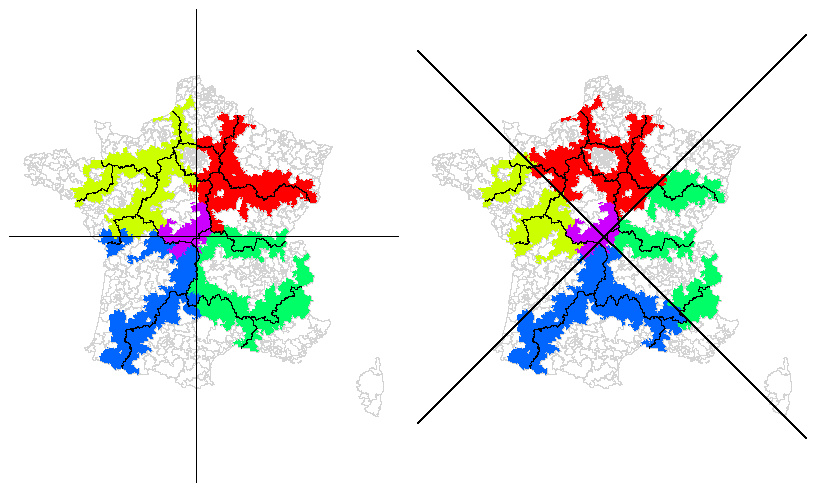
\includegraphics[scale=.7]{img/Methodo_decoupage.png}
\end{center}
\end{figure}
\emph{Source : calculs SDES}


On répartit ensuite le reste des communes dans les 4 cadrans du repère orthonormé ayant pour origine ce barycentre. Toutefois, les axes de ce repère passant le long de frontières, on conserve en partie l'effet frontière. Pour contourner ce biais, on effectue une rotation du repère orthonormé de 45 degrés.
Cette méthode fait néanmoins apparaître, selon les cas de figure, de très petites zones isolées, et des macro-zones qui ne sont pas d'un seul tenant. Une dernière étape consiste donc à rattacher les isolats à une macro-zone contiguë de taille suffisante, ou à séparer les parties non contiguës des grandes macro-zones.


\begin{figure}[H]
\caption{Découpage final en macro-zones}
\begin{center}
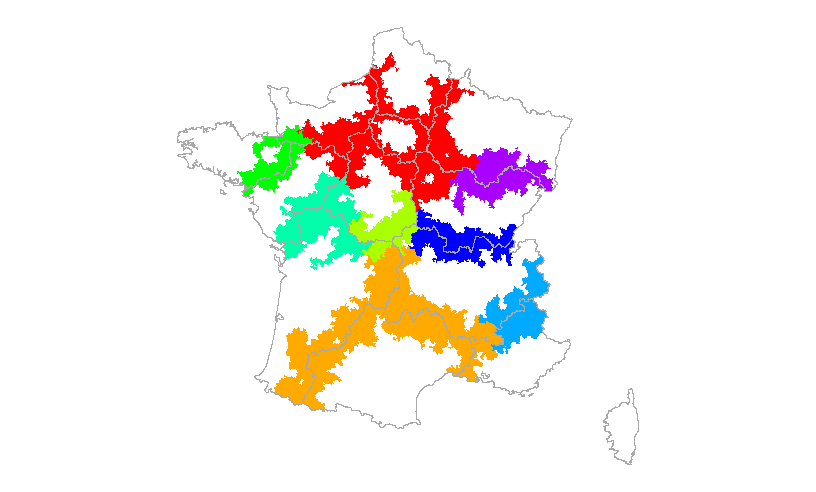
\includegraphics[scale=.7]{img/Decoupage.png}
\end{center}
\end{figure}
\emph{Source : calculs SDES}

\subsection{Les différentes simulations}

L'algorithme fonctionne à l'aide de deux paramètres qui permettent de faire varier le résultat final : le nombre de mailles finales souhaitées et une taille minimale (en termes de nombre de communes, de population, de nombre de logements...). 
\begin{itemize}
\item \'Etant donné que les travaux ont été menés région par région, c'est le nombre moyen de communes par maille qui a été utilisé pour déterminer le nombre final de mailles (pour que celui-ci soit homogène quelle que soit la taille de la région). Dans le cadre des exercices de simulation, ce nombre a varié entre 20 et 80.
\item Une taille minimum en termes de population. Deux seuils ont été testés pour chaque valeur du nombre de communes par maille : 40 000 et 50 000. Ces seuils ont été choisis pour que les mailles soient de taille significative et que des projections de populations puissent y être envisagées.
\end{itemize}

Après concertation avec les membres des comités, parmi ces 16 simulations, c'est le scénario fixant le nombre moyen de communes par maille à 40, avec une taille minimale de 40 000 habitants qui a été retenu, ce qui représente 777 mailles \emph{in fine}.

\subsection{Le traitement des îles}

L'algorithme fonctionne sur des ensembles contigus ; les îles ont donc été traitées à part. Deux cas de figure se sont présentés :
\begin{itemize}
\item Les îles composées d'une seule commune (par exemple l'île d'Yeu) ont été rattachées à la maille continentale la plus proche (au sens de la distance géographique)
\item Les îles composées de plusieurs communes (exemple : île d'Oléron) constituent des mailles autonomes
\end{itemize}


\section{Caractérisation des mailles}

Une fois défini le contour de ces mailles, les indicateurs initiaux ont été agrégés à cette nouvelle échelle. Pour caractériser ces marchés locaux, on effectue de nouveau une ACP suivie d'une classification qui permettent de dégager 6 types.

\subsection{L'habitat au premier plan}

Un des principaux résultats de ce travail est que ce nouveau maillage permet de mettre au premier plan les disparités territoriales liées à l'habitat. En effet, les indicateurs sélectionnés, pris à la maille communale, mettent en évidence, en premier lieu, les clivages traditionnels entre les territoires : ceux-ci se distinguent avant tout par leur degré d'urbanité, essentiellement retracé par la densité de population et leur position dans les catégories du zonages en aires urbaines. Le maillage habitat permet de mettre au premier plan les clivages relatifs aux caractéristiques des marchés locaux du logement.

\begin{figure}[H]
\caption{Disparités territoriales selon la maille}
\begin{center}
\begin{tabular}{c c}
Maille Communale & Maille logement \\
\hline
Degré d'urbanité & Degré de tension \\
Degré de tension & Taille des ménages \\
Zones touristiques & Zones touristiques \\
\hline
\end{tabular}
\end{center}
\end{figure}

C'est donc le degré de tension (défini par un pouvoir d'achat immobilier en retrait et une suroccupation des logements marquée) et la taille des ménages qui différencient le plus les mailles obtenues. 



\begin{figure}[H]
\caption{Indicateurs les plus discriminants}
\begin{center}
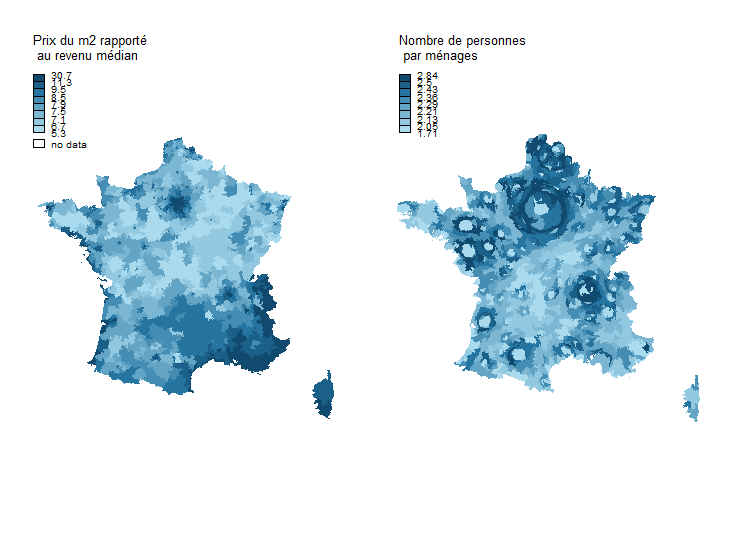
\includegraphics[scale=.8]{img/Discrim_mailles.png}
\end{center}
\end{figure}
\emph{Sources : calculs SDES d'après BIEN et PERVAL 2012, Filocom2013 et Insee, RP2014}

Les carte en figure 8 (notamment l'anamorphose) montrent la capacité du maillage à faire différencier les villes-centre des périphéries, ce qui n'est pas le cas pour les maillages d'études usuels.

\subsection{Typologie des mailles}

Ces disparités permettent de regrouper les marchés du logement en 6 grands types aux caractéristiques très distinctes :

\begin{enumerate}
\item Classe 1 : Mailles détendues à dominante rurale. Les mailles appartenant à cette catégorie sont marquées par les prix relatifs les plus bas (figure 3); parallèlement, le taux de vacance y est le plus élevé et le parc le plus ancien. Les ménages y sont également plus petits, et la durée d'occupation des logements est plus élevée que la moyenne. Les mailles de cette classe se trouvent essentiellement dans les espaces de faible densité, hors des zones de montagne, principalement le long de la diagonale Nord-Est / Sud-Ouest (figure 4). Leur empreinte sur le territoire est importante en termes de superficie, mais ces mailles regroupent un peu moins de 19 \% de la population.

\item Classe 2 : Mailles peu tendues des couronnes périurbaines. Les ménages sont plutôt de grande taille, la vacance y est faible. Ce groupe est le plus proche de la moyenne sur l'ensemble des indicateurs. Les prix y sont modérés relativement aux revenus, et la durée d'occupation plutôt élevée. La sur-occupation des logements et le taux de vacances sont eux en retrait. Ces mailles se situent essentiellement en périphérie des principales aires urbaines et dessinent le réseau inter-urbain ; Près de 29 \% de la population y réside.

\item Classe 3 : Mailles assez tendues des pôles urbains de province. Cette classe de mailles présentent un pouvoir d'achat immobilier un peu en retrait par rapport aux deux précédentes, proche de la moyenne nationale. En revanche, les ménages y sont significativement plus petits et la durée d'occupation en retrait. Ces mailles comptent relativement plus de logements sociaux que les deux types précédents. De fait, on les trouve au cœur des aires urbaines de provinces : ce sont donc des espaces urbains, où la population est plus jeune, donc avec une plus faible proportion de familles, ce qui explique la faible taille des ménages et le turnover plus important. Environ un quart de la population est regroupée dans cette classe.

\begin{figure}[H]
\caption{Indicateurs discriminants}
\begin{center}
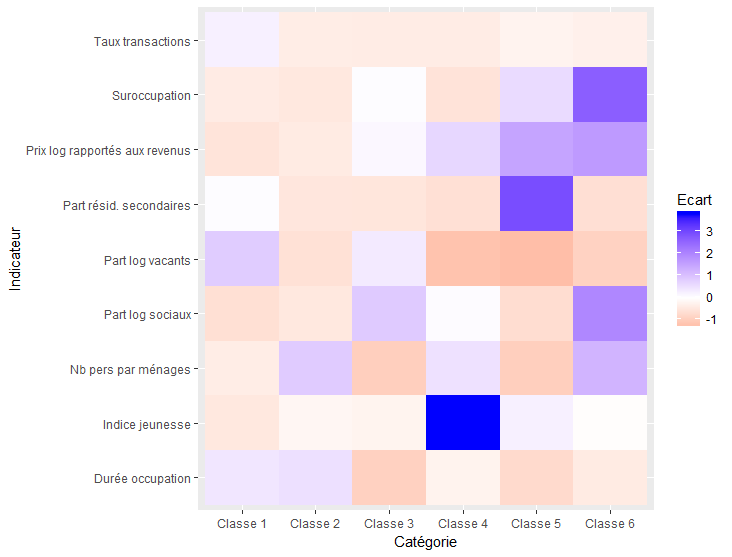
\includegraphics[scale=.8]{img/Caract_typo.png}
\end{center}
\end{figure}
\emph{Source : calculs SDES} \\
\emph{Lecture : La classe 4 se caractérise par un écart à la moyenne significatif et positif sur l'indice de jeunesse. La part de logements vacants est en revanche en retrait par rapport à la moyenne nationale dans les classes 4 et 5} \\
\item Classe 4 : Mailles tendues des couronnes des aires urbaines attractives.  Ces mailles sont en très petit nombre, mais sont très spécifique : le parc de logement y est très récent par rapport aux autres et le pouvoir d’achat en retrait par rapport aux 3 classes précédentes. Par ailleurs, la taille des ménages est plutôt importante et la sur-occupation nettement en retrait. Elles se situent dans les espaces périurbains proches des aires urbaines dont la population a fortement crû ces dernières années. Par exemple, on y trouve l’entière banlieue de Toulouse, mais également la périphérie ouest de Bordeaux ou encore l’est de Lyon. L’attractivité résidentielle de ces mailles a donc conduit à des flux de construction de logements importants, mais s’est également traduit par un accroissement des prix. Elles regroupent seulement 2\% de la population.

\item Classe 5 : Mailles tendues des espaces touristiques. Cette classe présente avant tout un pouvoir d’achat immobilier en retrait : les prix y sont élevés relativement aux revenus des habitants et un taux de sur-occupation plus élevé. La caractéristique principale est avant tout la forte part de résidences secondaires qu’on y trouve. De fait, ces mailles se situent dans les espaces à vocation touristique, littoraux et montagnards. Le marché des résidences secondaire y pousse les prix à la hausse et accroît le décalage avec les revenus des résidents, ce qui leur confère les caractéristiques de marchés tendus. Ces mailles regroupent environ 7\% de la population.

\item Classe 6 : Mailles à difficultés prononcées d’accès au logement. Ce dernier groupe contient les marchés les plus tendus : le pouvoir d’achat immobilier y est nettement en retrait, et le taux de sur-occupation des logements est élevé, tout comme le nombre de personnes par ménages. On y trouve également la plus forte proportion de logements sociaux. Ces mailles correspondent aux marchés tendus d’Île de France, ainsi que ceux où le pouvoir d’achat immobilier des ménages est en retrait du fait de faibles revenus (Roubais, Marseille). 18,4\% de la population réside dans ces marchés dont l’empreinte géographique est toutefois très restreinte.
\end{enumerate}

\begin{figure}[H]
\caption{Indicateurs discriminants}
\begin{center}
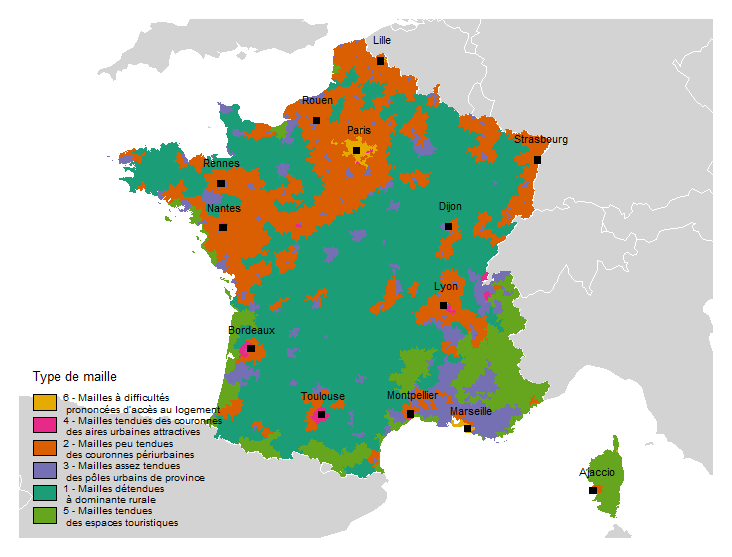
\includegraphics[scale=.8]{img/Typo_mailles.png}
\end{center}
\end{figure}
\emph{Source : calculs SDES}

\subsection{Cohésion et dynamique de ces mailles}

\subsubsection{Cohésion}

La typologie précédente permet de mettre en évidence les grandes disparités qui traversent les différents marchés du logement. Mais ces marchés présentent de l'hétérogénéité également entre les communes qui les composent. Le score de diversité \footnote{Pour mesurer les disparités entre les communes au sein d'un même marché du logement (maille), on calcule un score de diversité : il s'agit de la somme des écarts-types, calculés sur chacun des indicateurs (qui ont été centrés-réduits au préalable). Plus ce score est élevé, plus l'hétérogénéité de la maille considérée est importante. Certaines mailles n'étant constituées que d’une seule commune (généralement les villes-centres des aires urbaines), ce score n'est pas calculable.} montre des spécificités territoriales marquées. En premier lieu, les communes dans l'urbain et le périurbain sont plus homogènes que les espaces de faible densité démographique. Par ailleurs, les mailles de la classe correspondant aux espaces à vocation touristique présentent une forte hétérogénéité interne (figure 5) c'est le cas par exemple de la Normandie et du plateau de Langres. Une partie de la couronne périurbaine de Paris, à l'exception de l'Ouest présente également des marchés très disparates. A l'opposé, l'Ouest du pays apparaît plus homogène, notamment la Bretagne et les Pays de la Loire. Le département du Nord, ainsi que l'Alsace et le Lyonnais présentent également de moindres disparités internes.

\begin{figure}[H]
\caption{Score de diversité}
\begin{center}
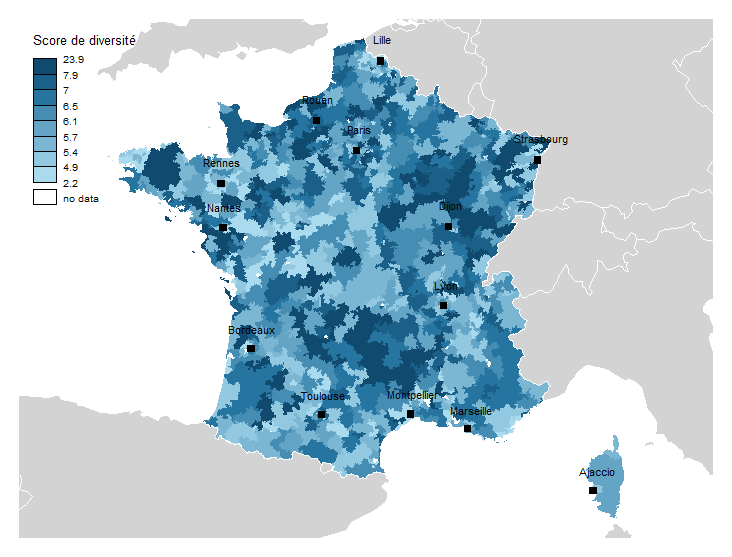
\includegraphics[scale=.8]{img/Diversite.png}
\end{center}
\end{figure}
\emph{Source : calculs SDES}

\subsubsection{Dynamiques}

L'analyse statique des indicateurs permet donc de mettre en évidence des disparités inter et intra-mailles. L'analyse de ces indicateurs en évolution montre la dynamique de ces espaces. Or, la corrélation entre les indicateurs pris en stock (c'est à dire à un instant T) et en évolution est systématiquement positive : la diagonale de la figure 6 illustre ces corrélations. Cela signifie donc que la trajectoire des marchés du logement est étroitement liée à leur situation. En d'autres termes, les caractéristiques de ces marchés ont tendance à se renforcer dans le temps. Par exemple, il existe une forte corrélation entre le niveau du pouvoir d'achat immobilier (prix rapportés aux revenus) et son évolution au cours du temps, ce qui signifie que les prix ont le plus progressé dans les mailles où ils sont les plus élevés. Le constat est similaire pour la durée d'occupation des logements qui a progressé là où elle était déjà élevée. Sur les autres indicateurs, la corrélation est plus faible, mais toujours positive.

\begin{figure}[H]
\caption{Corrélation entre indicateurs de stock et indicateurs de flux}
\begin{center}
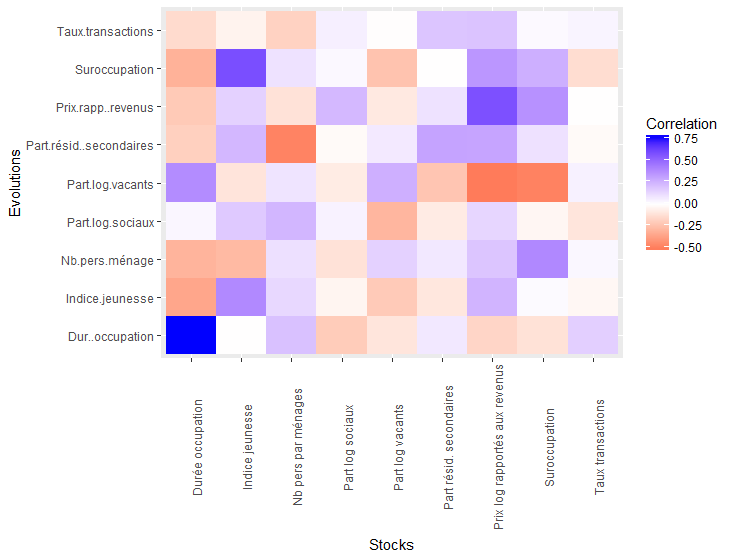
\includegraphics[scale=.8]{img/Dynam.png}
\end{center}
\end{figure}
\emph{Source : calculs SDES}

\nocite{*}
%\bibliographystyle{acm}
%\bibliography{DB}

\end{document}  